% Provenance (never printed): see sources/outline_sources.md (Year 1: solute and particle
% fluxes; the Hjulstrom diagram; settling velocity; denudation rates). Exercise and problem
% values in the Book 3 scratch calculator calc/ch20.py; figure data from
% figdata/bachelor-1/settling.py and threshold.py. Erosion, transport and deposition are
% Book 1's (g5); the sediment load in three forms, the denudation rate and isostatic rebound
% are Book 2's (g12), re-founded here (load, denudation rate) or recalled (rebound); discharge
% and the drainage basin are Book 2 g10's; Airy isostasy is ch. 11's; viscosity, Stokes' law
% and the Reynolds number are the physics books' (admitted, pointer). Grain-size classes and
% sorting belong to ch. 21.
\chapter{Erosion and Transport}\label{ch:b1:erosion-transport}

After a storm the river under the bridge runs brown. The water that was clear
the day before is thick with mud, swirls around the piers and carries
branches, and on the bed, unseen, pebbles knock against each other as they
roll. Each second the flood takes tonnes of the land with it. Downstream,
behind a dam, the same mud settles in the still water of the reservoir, which
loses a little of its volume every year; farther still, at the river's mouth,
it spreads into the sea as a brown plume that can be seen from space. This
chapter puts numbers on that journey: how much a river carries and in what
forms, how fast a grain sinks, what current it takes to set it moving, and how
fast, in the end, a whole landscape is worn away.

\begin{recall}
Erosion is the wearing-away of the land and the carrying-away of the pieces;
deposition is their laying-down where the carrier slows (Book~1, grade~5). A
river carries its sediment load as \omterm{def:b1:erosion-transport:load}{bed load}, \omterm{def:b1:erosion-transport:load}{suspended load} and \omterm{def:b1:erosion-transport:load}{dissolved
load}; the \omterm{def:b1:erosion-transport:denudation}{denudation rate} of a region is the thickness of rock removed from it
per unit time, in metres per million years; when erosion removes a thickness
$e$ of \omterm{def:b1:layered-earth:layers}{crust}, isostatic rebound lets the surface go down by only
$e(1 - \rho_c/\rho_m)$ (Book~2, grade~12). The discharge of a river is the
volume of water that passes a cross-section per unit time, and its drainage
basin the area that supplies it (Book~2, grade~10). In \omterm{prop:b1:isostasy-gravity:airy}{Airy isostasy} the \omterm{def:b1:layered-earth:layers}{crust}
floats on the \omterm{def:b1:layered-earth:layers}{mantle} with a root proportional to its relief
(\cref{prop:b1:isostasy-gravity:airy}). The \omterm{def:b1:weathering-clays:hydrolysis}{hydrolysis} of silicates sends ions
and dissolved silica to the rivers (\cref{def:b1:weathering-clays:hydrolysis}).
The dynamic viscosity $\mu$ of a fluid measures its resistance to shearing,
and the kinematic viscosity is $\nu = \mu/\rho$; a sphere of diameter $d$
moving slowly at the speed $w$ through a fluid feels the drag $3\pi\mu d w$
(Stokes' law); the Reynolds number $w d/\nu$ compares inertia with viscous
forces, and the flow around the sphere is smooth while it stays small (the
physics books).
\end{recall}

\section{Solute and particle fluxes}\label{sec:b1:erosion-transport:fluxes}

A river removes the land in two ways: as matter in solution, the products of
\omterm{def:b1:weathering-clays:weathering}{chemical weathering}, and as solid grains, the products of \omterm{def:b1:weathering-clays:weathering}{physical weathering}
and the insoluble residues of \omterm{def:b1:weathering-clays:weathering}{chemical weathering}. The two travel differently,
and the grains themselves travel in two ways.

\begin{definition}[Dissolved load, suspended load, bed load]\label{def:b1:erosion-transport:load}
The load of a river is the matter it carries past a cross-section, in three
parts that differ by how they travel. The \emph{dissolved load}\index{dissolved
load} is the matter in solution, ions and dissolved silica, which moves with
the water at its own speed. The \emph{suspended load}\index{suspended load} is
made of grains held up within the flow by its turbulence, mostly clay, silt
and fine sand, which move at nearly the speed of the water and seldom touch
the bed. The \emph{bed load}\index{bed load} is made of grains that roll, slide
or hop along the bed, in frequent contact with it, much more slowly than the
water.
\end{definition}

\begin{omfigure}
\begin{tikzpicture}[font=\footnotesize, >={Stealth[length=4pt]}]
% schematic: the three loads of a river (side view) and the forces on a bed grain
\fill[omDef!12] (0,0) rectangle (9,3.2);
\draw[omDef!80!black, thick] (0,3.2) -- (9,3.2);
\node[anchor=south west, omDef!80!black] at (0,3.2) {water surface};
% flow profile arrows (velocity grows upward)
\foreach \y/\l in {0.35/0.5, 0.8/0.9, 1.4/1.15, 2.1/1.3, 2.8/1.4} {\draw[->, black!55] (0.25,\y) -- ++(\l,0);}
\draw[black!55] (0.25,0.12) -- (0.25,3.05);
\node[anchor=north west, black!65, align=left] at (0.2,-0.15) {flow velocity\\ profile};
% bed
\fill[black!12] (0,-0.05) rectangle (9,0.12);
\foreach \x in {0.1,0.45,...,8.9} {\fill[black!45] (\x,0.0) circle[radius=0.09];}
% dissolved load: ions
\foreach \x/\y/\s in {2.3/2.7/+, 3.1/1.9/-, 4.0/2.85/+, 4.7/2.2/-, 5.6/2.75/+, 6.3/1.85/+, 7.2/2.6/-, 8.2/2.2/+, 2.7/1.2/-, 7.8/1.3/-} {\node[circle, draw=omThm, inner sep=0.2pt, minimum size=7pt, font=\tiny, text=omThm] at (\x,\y) {$\s$};}
% suspended load: fine grains, denser near the bed
\foreach \x/\y in {2.1/1.5, 2.6/0.9, 3.0/2.5, 3.4/0.6, 3.7/1.4, 4.2/0.8, 4.4/1.9, 4.9/0.55, 5.2/1.2, 5.5/2.1, 5.9/0.7, 6.1/1.5, 6.6/0.9, 6.9/2.3, 7.4/0.6, 7.6/1.7, 8.0/0.85, 8.5/1.4, 3.9/0.45, 5.0/0.35, 6.4/0.4, 2.4/0.45, 8.6/0.5} {\fill[brown!75!black] (\x,\y) circle[radius=0.05];}
% bed load: rolling and hopping grains
\fill[black!60] (3.2,0.27) circle[radius=0.15];
\draw[->, black!70] (3.0,0.55) arc[start angle=150, end angle=30, radius=0.25];
\fill[black!60] (5.6,0.25) circle[radius=0.12];
\draw[->, black!70, densely dashed] (4.6,0.2) .. controls (4.9,0.9) and (5.3,0.7) .. (5.55,0.4);
\fill[black!60] (4.6,0.22) circle[radius=0.06];
% labels
\node[omThm, anchor=west] at (9.2,2.5) {dissolved load: ions};
\node[brown!75!black, anchor=west] at (9.2,1.5) {suspended load:};
\node[brown!75!black, anchor=west] at (9.2,1.1) {clay, silt, fine sand};
\node[black!75, anchor=west] at (9.2,0.4) {bed load: rolling,};
\node[black!75, anchor=west] at (9.2,0.0) {sliding, hopping grains};
\draw[->, thick, black!70] (6.8,3.55) -- node[above] {flow} (8.6,3.55);
% inset: forces on a grain resting on two others; it pivots about its downstream contact
\begin{scope}[xshift=11.8cm, yshift=-2.2cm]
  \fill[black!12] (-1.2,-0.4) rectangle (1.2,0);
  \fill[black!40] (-0.6,-0.15) circle[radius=0.28]; \fill[black!40] (0.6,-0.15) circle[radius=0.28];
  \fill[black!65] (0,0.166) circle[radius=0.4];
  \draw[->, thick, omDef!80!black] (0,0.166) -- (0,1.15) node[above] {lift};
  \draw[->, thick, omThm] (0,0.166) -- (1.05,0.166) node[right] {drag};
  \draw[->, thick, black] (0,0.166) -- (0,-0.8) node[below] {submerged weight};
  \draw[->, thick, black!60] (-1.4,0.85) -- (-0.5,0.85) node[pos=0, left] {flow};
  \fill[red!60!black] (0.353,-0.020) circle[radius=0.045];
  \node[font=\scriptsize, anchor=north west, black!70] at (0.5,-0.4) {pivot};
\end{scope}
\end{tikzpicture}

{\small The three loads of a river, seen from the side (schematic, not to
scale). The flow is fastest near the surface and slows to zero at the bed. Ions
are spread through the whole depth; suspended grains are carried by the eddies,
more of them near the bed; bed-load grains roll, slide or make short hops.
Right: the forces on a grain of the bed. The drag and lift of the flow tend to
roll it over its downstream neighbour, about the contact point; its weight in
the water holds it back.}
\label{fig:b1:erosion-transport:loads}
\end{omfigure}

The boundary between the two solid loads is not fixed by the grain size: it
depends on the flow. A flood that carries sand in suspension leaves it on the
bed, as \omterm{def:b1:erosion-transport:load}{bed load}, when it wanes; the finest clay, on the other hand, stays in
suspension in almost any current and is hardly ever found on the bed of a
flowing river. Each load is measured as a flux, a mass per unit time through a
cross-section of the river.

\begin{proposition}[Flux of a load]\label{prop:b1:erosion-transport:flux}
Let $c$ be the concentration of a dissolved or \omterm{def:b1:erosion-transport:load}{suspended load} (mass per unit
volume of water) and $u$ the velocity of the water, both varying across the
section of area $A$. (1)~The instantaneous flux of the load through the
section is
\[
  F = \iint_A c\,u\,\mathrm dA = \overline{c}_Q\,Q,
\]
where $Q = \iint_A u\,\mathrm dA$ is the discharge and $\overline{c}_Q$ the
mean concentration weighted by the velocity. (2)~Over a period $T$ in which the
discharge $Q(t)$ and the concentration $C(t)$ of the river vary, the mass
carried is
\[
  M = \int_0^T Q\,C\,\mathrm dt = T\left(\overline{Q}\;\overline{C} +
  \operatorname{cov}(Q, C)\right),
\]
where the bars are means over time and $\operatorname{cov}(Q, C)$ is the mean
of $(Q - \overline{Q})(C - \overline{C})$. The product of the mean discharge
and the mean concentration gives the right mass only if the two are
uncorrelated.
\end{proposition}

\begin{proof}
(1)~In a time $\mathrm dt$ the water crossing a small area $\mathrm dA$ of the
section fills a volume $u\,\mathrm dA\,\mathrm dt$, which carries the mass
$c\,u\,\mathrm dA\,\mathrm dt$; summing over the section gives $F$, and
$\overline{c}_Q$ is defined as $F/Q$. (2)~Write $Q = \overline{Q} + Q'$ and $C =
\overline{C} + C'$, where the fluctuations $Q'$ and $C'$ have zero mean over the
period. Then $QC = \overline{Q}\,\overline{C} + \overline{Q}\,C' + Q'\,\overline{C}
+ Q'C'$; the two middle terms average to zero, and the mean of $Q'C'$ is the
covariance.
\end{proof}

The covariance matters for the \omterm{def:b1:erosion-transport:load}{suspended load}. Its concentration rises steeply
in floods, when the rain washes soil into the streams and the faster flow lifts
grains from the bed, so $Q$ and $C$ grow together: a large part of a river's
yearly sediment passes in a few days of flood, and a sampling campaign that
misses them, or a mean concentration multiplied by the mean discharge,
underestimates the load. The \omterm{def:b1:erosion-transport:load}{dissolved load} behaves the other way: floods
dilute it, and its concentration is highest at low flow, when the river is fed
by ground water that has been in long contact with the rock.

\begin{method}[The yearly load of a river from gauging]\label{met:b1:erosion-transport:gauging}
\begin{enumerate}
  \item Record the discharge continuously at a gauging station.
  \item Sample the water at many discharges, floods included, and measure the
        mass of sediment per litre (by filtering and weighing) and of each
        dissolved species.
  \item Weight the concentrations by the discharge at the time of sampling to
        get the flow-weighted mean concentration, or fit the concentration as
        a function of the discharge and apply it to the whole record.
  \item Multiply by the total volume of water of the year, or sum $Q\,C\,\Delta
        t$ over the record (\cref{prop:b1:erosion-transport:flux}).
  \item Add the \omterm{def:b1:erosion-transport:load}{bed load}, which water samplers miss, from separate
        measurements or as an estimated fraction.
  \item For the \omterm{def:b1:erosion-transport:load}{dissolved load}, remove what does not come from the rock: the
        salts brought by rain and, for the bicarbonate, the carbon taken from
        the air (\cref{ch:b1:weathering-clays}).
\end{enumerate}
\end{method}

\begin{omfigure}
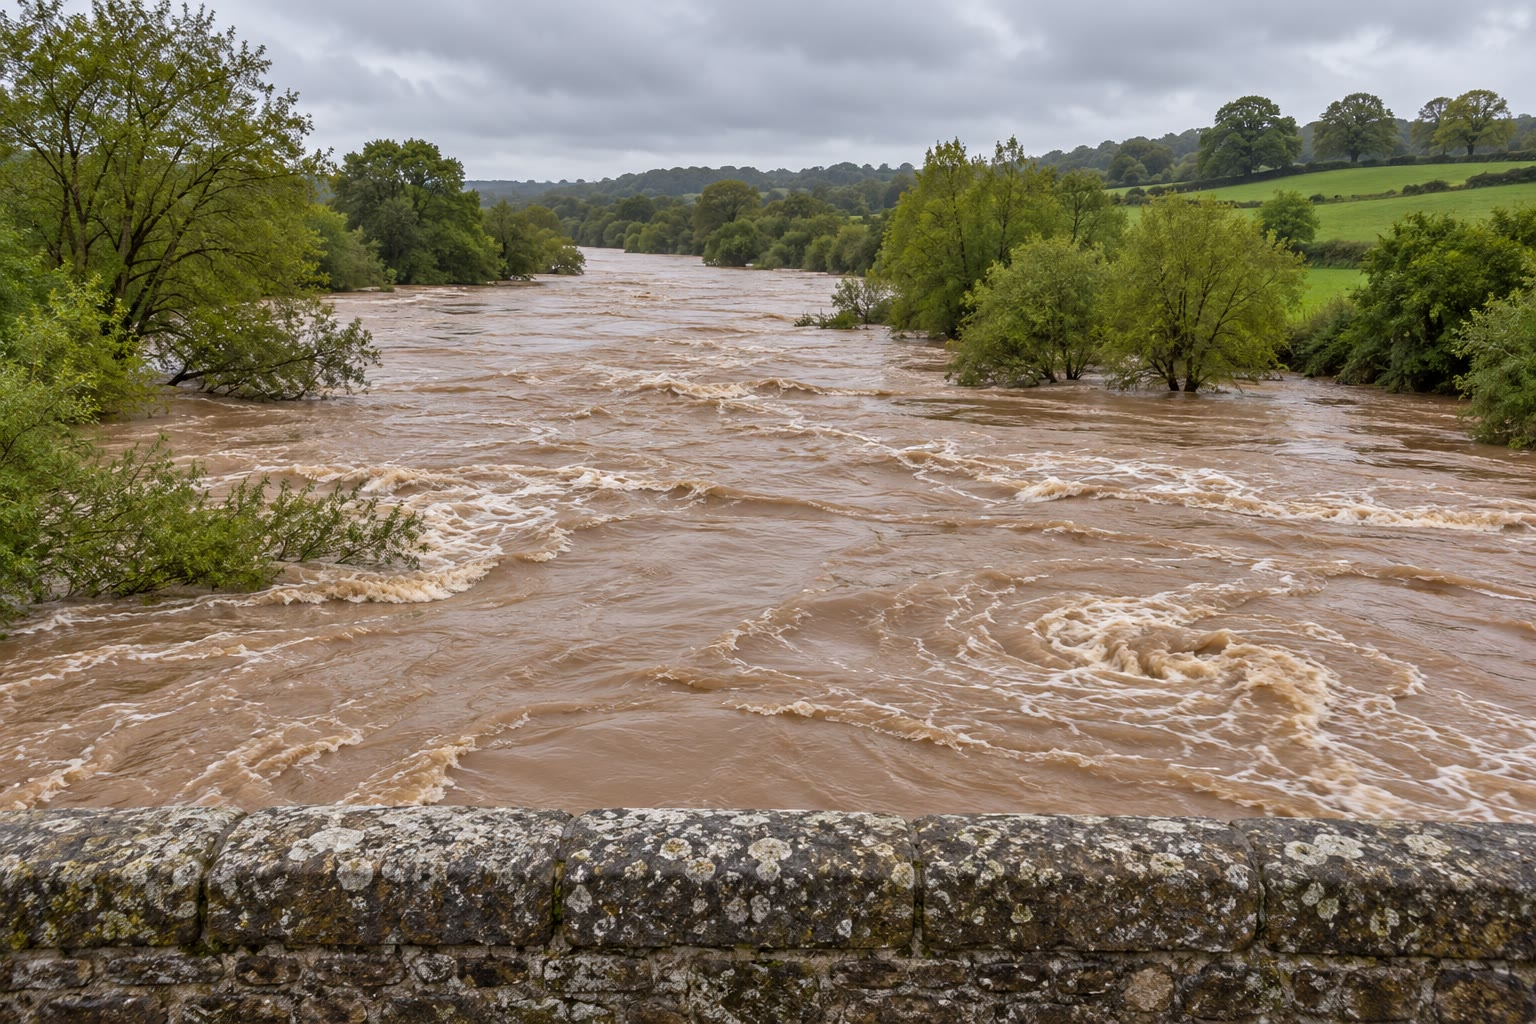
\includegraphics[height=5.1cm]{images/book3/ai/b1-muddy-river.jpg}\hfill
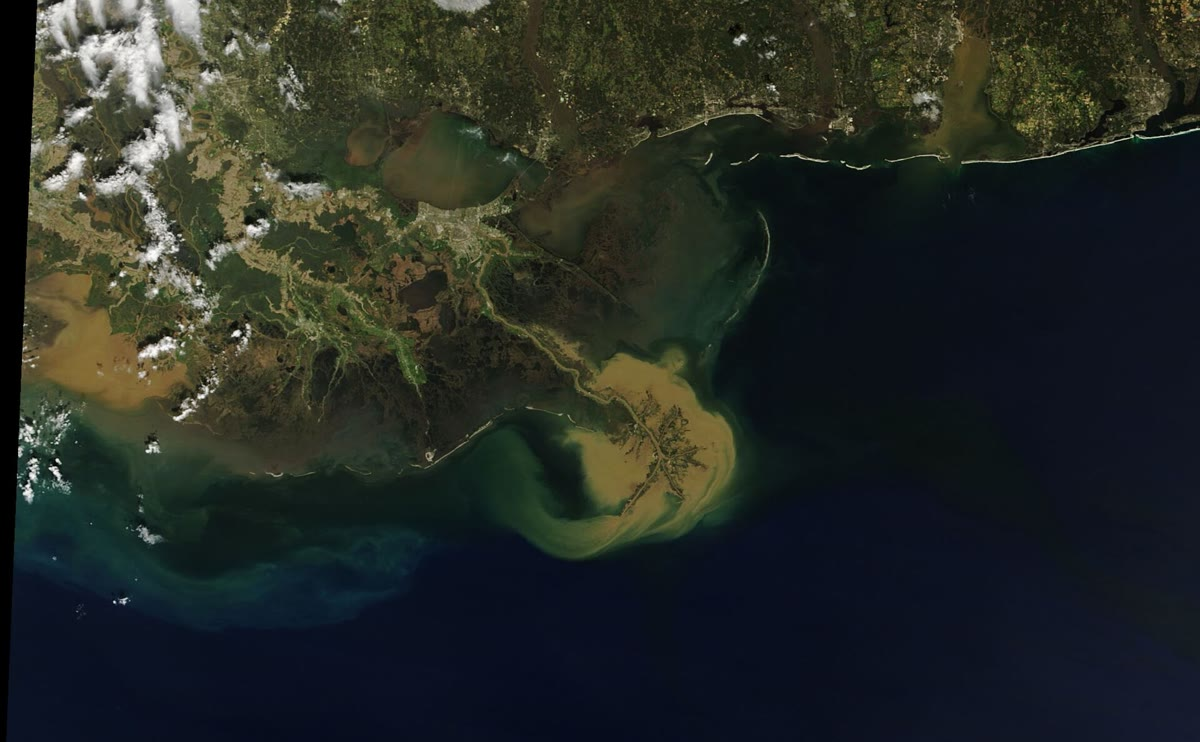
\includegraphics[height=5.1cm]{images/book3/b1-mississippi-plume.jpg}
\par\smallskip{\small Left: a river in flood carries brown, sediment-laden
water (AI illustration). Right: the flood plume of the Mississippi spilling
into the Gulf of Mexico around its delta, seen by the MODIS instrument on the
Terra satellite on 4~March 2018; the suspended mud colours the sea brown and
green, and the southeast wind pushes the plume to the northwest. NASA Earth Observatory image by Joshua Stevens, public domain, via
Wikimedia Commons.}
\label{fig:b1:erosion-transport:plume}
\end{omfigure}
% ledger: commons:mississippi-plume

\emph{The world's rivers.} Before any human influence, the rivers of the world
carried an estimated \qty{14}{Gt} of suspended sediment a year to the coastal
ocean, \qty{15.5}{Gt} with the \omterm{def:b1:erosion-transport:load}{bed load}. People have changed both ends of the
journey: farming and deforestation have raised soil erosion, adding about
\qty{2.3}{Gt} a year to the rivers, while reservoirs hold back sediment: the
large ones trap about \qty{20}{\percent} of the flux and the small ones another
\qty{6}{\percent}, and more than \qty{100}{Gt} of sediment now lies behind
dams built mostly in the past fifty years. The net effect is a reduction: the
modern flux is about \qty{12.6}{Gt} a year.
% ledger: syvitski:flux

\begin{dated}{2005}
The figures for the suspended sediment flux, before and after human influence,
come from a global model of river sediment published in 2005. Dams have been
built since.
\end{dated}
% ledger: syvitski:flux

The \omterm{def:b1:erosion-transport:load}{dissolved load} is smaller. A classic compilation of river analyses, made in
1963, put the dissolved matter that the rivers of the world deliver to the sea
at about \qty{3.9}{Gt} a year, about \qty{30}{\percent} of the modern suspended
flux, at a mean concentration of \qty{120}{mg} per litre. Bicarbonate makes
nearly half of it, \qty{58}{mg.L^{-1}}, followed by calcium, silica, sulfate,
chloride and sodium. Part of it does not come from the rock: much of the
bicarbonate carries carbon drawn from the air or the soil, and part of the
chloride and sodium comes from sea salt carried by rain. Individual rivers range
widely around these means.
% ledger: livingstone:world-dissolved, syvitski:flux

\emph{The sediment budget of a basin.} Not every grain eroded in a drainage
basin reaches its outlet. Soil washed from a field may stop at the foot of the
slope, sand may be stored for centuries in the floodplain and the river's bars,
and a reservoir may hold back most of what enters it. The load measured at the
outlet is the balance of the budget: what is eroded on the slopes and from the
banks, minus what is stored on the way, plus what is taken back from old
stores. Over a few decades of gauging this balance can be far from the
long-term rate of erosion, in either direction, which is one reason for the
other methods of \cref{sec:b1:erosion-transport:denudation}.

\section{Settling velocity}\label{sec:b1:erosion-transport:settling}

A grain is denser than water and sinks. Whether a river can carry it, and
where it will be deposited, depends first on how fast it sinks.

\begin{definition}[Settling velocity]\label{def:b1:erosion-transport:settling}
The \emph{settling velocity}\index{settling velocity} $w_s$ of a grain is the
constant velocity at which it falls through still water, when the drag of the
water balances its submerged weight, its weight minus the buoyancy of the
water it displaces.
\end{definition}

A grain released in still water accelerates until its drag, which grows with
its speed, balances its submerged weight; for a grain of sand or silt this
takes a small fraction of a second, so the \omterm{def:b1:erosion-transport:settling}{settling velocity} is the speed at
which it falls nearly all the way. With the densities $\rho_s$ of the grain
and $\rho$ of the water, write $R = (\rho_s - \rho)/\rho$ for the relative
submerged density.

\begin{proposition}[Stokes settling]\label{prop:b1:erosion-transport:stokes}
A sphere of diameter $d$ and density $\rho_s$ falling slowly through water of
density $\rho$ and dynamic viscosity $\mu$, under Stokes' law, has the \omterm{def:b1:erosion-transport:settling}{settling
velocity}
\[
  w_s = \frac{(\rho_s - \rho)\,g\,d^2}{18\,\mu} = \frac{R\,g\,d^2}{18\,\nu}.
\]
The law holds while the grain Reynolds number $w_s d/\nu$ is below about 1,
that is, for diameters below $d_1 = \left(18\,\nu^2/(R\,g)\right)^{1/3}$.
\end{proposition}

\begin{proof}
The weight of the sphere is $\rho_s g\,\pi d^3/6$ and the buoyancy
$\rho g\,\pi d^3/6$, so its submerged weight is $(\rho_s - \rho)\,g\,\pi d^3/6$.
At the \omterm{def:b1:erosion-transport:settling}{settling velocity} it equals the drag $3\pi\mu d\,w_s$:
\[
  (\rho_s - \rho)\,g\,\frac{\pi d^3}{6} = 3\pi\mu d\,w_s
  \quad\Longrightarrow\quad
  w_s = \frac{(\rho_s - \rho)\,g\,d^2}{18\,\mu},
\]
and dividing the numerator and the denominator by $\rho$ gives the second form.
The Reynolds number of this velocity is $R g d^3/(18\nu^2)$, which equals 1 for
$d = d_1$ and grows as $d^3$.
\end{proof}

For quartz, of density \qty{2650}{kg.m^{-3}}, in water at \qty{20}{\celsius},
of density \qty{998.2}{kg.m^{-3}} and viscosity \qty{1.0016}{mPa.s}: $R =
1.65$, $\nu = \qty{1.003e-6}{m^2.s^{-1}}$, and with $g =
\qty{9.81}{m.s^{-2}}$ the limit is $d_1 = \qty{0.104}{mm}$, a fine sand. Below
it, Stokes' law gives the settling velocities of silt and clay: a silt grain
\qty{10}{\micro m} across sinks at \qty{9.0e-5}{m.s^{-1}}, \qty{1}{m} in about
three hours; a clay particle of \qty{2}{\micro m} at
\qty{3.6e-6}{m.s^{-1}}, \qty{1}{m} in \num{3.2}~days. Natural clay particles are
flakes, not spheres, and sink still more slowly. Water \qty{5}{m} deep, perfectly
still, would take sixteen days to clear of such clay; a flowing river, whose
eddies keep stirring it up, never does, which is why the finest mud travels
to the sea.
% ledger: hom:quartz, nist:water, const:gn

Above $d_1$ the drag grows faster than in proportion to the velocity: the water
flowing past the grain separates behind it into a wake, and at large Reynolds
numbers the drag is proportional to the square of the velocity. Experiments on
natural grains are summed up in a single formula that joins the two regimes.

\begin{proposition}[Combined settling law]\label{prop:b1:erosion-transport:combined}
The \omterm{def:b1:erosion-transport:settling}{settling velocity} of natural grains of sieve diameter $d$ is, for all
sizes,
\[
  w_s = \frac{R\,g\,d^2}{C_1\,\nu + \sqrt{0.75\,C_2\,R\,g\,d^3}},
\]
with $C_1 = 18$ and $C_2 = 1.0$.
\end{proposition}
\admitted
% ledger: fc:settling

The law is due to Ferguson and Church, who fitted it to measured settling
velocities of natural sands. For small grains the square root is
negligible and it reduces to Stokes' law; for large grains the first term of
the denominator is negligible and $w_s \to \sqrt{4 R g d/(3 C_2)}$, which grows
only as the square root of the size. The constants depend on the shape of the
grains: $C_2 = 0.4$ describes smooth spheres, larger values more angular
grains, which meet more drag. The two laws part company above
\qty{0.1}{mm}. For a grain of \qty{1}{mm} the combined law gives
\qty{0.126}{m.s^{-1}}, seven times less than Stokes' law; for a pebble of
\qty{10}{mm}, \qty{0.46}{m.s^{-1}} against a meaningless \qty{90}{m.s^{-1}}
(diagram below).
% ledger: fc:settling

\begin{omfigure}
\begin{tikzpicture}[font=\small]
% settling velocity of quartz grains in water at 20 C (figdata/bachelor-1/settling.py)
\begin{axis}[width=11cm, xmode=log, ymode=log, xmin=0.001, xmax=10, ymin=1e-8, ymax=10, height=8cm,
    xlabel={grain diameter $d$ (\si{mm})}, ylabel={settling velocity (\si{m.s^{-1}})},
    ytick={1e-8,1e-6,1e-4,1e-2,1},
    legend style={at={(0.03,0.97)}, anchor=north west, font=\footnotesize}, legend cell align=left,
    grid=major, grid style={black!10}]
  \addplot[omDef, thick, dashed] table[x=d_mm, y=w_stokes] {figdata/out/bachelor-1-settling-curves.dat};
  \addplot[omThm, very thick] table[x=d_mm, y=w_fc] {figdata/out/bachelor-1-settling-curves.dat};
  \legend{Stokes' law, combined law (natural grains)}
  \draw[black!55, densely dotted] (axis cs:0.1037,1e-7) -- (axis cs:0.1037,10);
  \node[font=\scriptsize, anchor=west, align=left, black!75] at (axis cs:0.115,1e-6) {grain Reynolds\\ number $= 1$};
  \node[font=\scriptsize, black!70] at (axis cs:0.002,3e-8) {clay};
  \node[font=\scriptsize, black!70] at (axis cs:0.016,3e-8) {silt};
  \node[font=\scriptsize, black!70] at (axis cs:0.35,3e-8) {sand};
  \node[font=\scriptsize, black!70] at (axis cs:4.5,3e-8) {gravel};
  \draw[black!40] (axis cs:0.0039,1e-8) -- (axis cs:0.0039,1e-7);
  \draw[black!40] (axis cs:0.0625,1e-8) -- (axis cs:0.0625,1e-7);
  \draw[black!40] (axis cs:2,1e-8) -- (axis cs:2,1e-7);
\end{axis}
\end{tikzpicture}

{\small \omterm{def:b1:erosion-transport:settling}{Settling velocity} of quartz grains in water at \qty{20}{\celsius}
against their diameter, both on logarithmic scales: Stokes' law and the
combined law of natural grains, computed. On these scales Stokes' law is a
straight line of slope 2. The two agree for silt and clay; above about
\qty{0.1}{mm}, where the grain Reynolds number passes 1, the drag of the wake
slows the coarse grains. The ticks at the bottom mark the boundaries of the
grain-size classes, at \qty{3.9}{\micro m} ($1/256$~mm), \qty{62.5}{\micro m}
($1/16$~mm) and \qty{2}{mm}.}
\label{fig:b1:erosion-transport:settling}
\end{omfigure}
% ledger: fc:settling, usgs:wentworth-phi

Over the range of the diagram, from the finest clay to a coarse gravel, the
\omterm{def:b1:erosion-transport:settling}{settling velocity} spans eight orders of magnitude. This is the first reason why
rivers sort their sediment: a slackening current drops its gravel at once, its
sand within metres, its silt within kilometres, and carries its clay to a
lake or to the sea. The grain-size classes and the sorting of sediments are
the subject of the next chapter (\cref{ch:b1:clastic-sediments}).

\section{Threshold of motion and the Hjulström diagram}\label{sec:b1:erosion-transport:threshold}

A grain at rest on the bed of a river is set moving by the force of the water
flowing over it. That force is measured by a stress.

\begin{definition}[Bed shear stress, shear velocity]\label{def:b1:erosion-transport:bed-shear}
The \emph{bed shear stress}\index{bed shear stress} $\tau_b$ of a flow is the
force per unit area that it exerts on its bed, parallel to the bed, in the
direction of the flow. The shear velocity is $u_* = \sqrt{\tau_b/\rho}$, a
velocity that measures the same stress.
\end{definition}

The \omterm{def:b1:erosion-transport:bed-shear}{bed shear stress} cannot be read from a current meter, but in a steady flow
it follows from a balance of forces.

\begin{proposition}[Depth--slope product]\label{prop:b1:erosion-transport:depth-slope}
In a steady, uniform flow of depth $h$ down a wide channel of small slope $S$,
the \omterm{def:b1:erosion-transport:bed-shear}{bed shear stress} is
\[
  \tau_b = \rho\,g\,h\,S .
\]
\end{proposition}

\begin{proof}
Consider the water above a piece of bed of length $L$ along the flow and of
unit width, the channel being so wide that its banks can be ignored. The flow
is steady and uniform, so this water does not accelerate and the forces on it
balance. The pressure forces on its upstream and downstream faces are equal and
opposite, since the depth is the same on both. Along the flow there remain the
component of the weight, $\rho g h L \sin\beta$, where $\beta$ is the angle of
the bed, and the friction of the bed, $\tau_b L$, opposed to it. Hence $\tau_b
= \rho g h \sin\beta$, and for a small angle $\sin\beta \approx \tan\beta = S$.
\end{proof}

A river \qty{2}{m} deep on a slope of \num{0.001}, a metre of fall per
kilometre, has $\tau_b = 998.2 \times 9.81 \times 2 \times 0.001 =
\qty{19.6}{Pa}$, and a shear velocity of \qty{0.140}{m.s^{-1}}. In a channel
that is not wide, the banks take their share of the friction, and the depth is
replaced by the hydraulic radius, the area of the section divided by its wetted
perimeter (\cref{exo:b1:erosion-transport:5}).

\emph{Forces on a grain.} The flow pushes a grain of the bed by its drag and
lifts it by the faster flow over its top (the inset of the first figure of this
chapter). Both forces act on the area of the grain, so they scale as $\tau_b
d^2$; the grain resists by its submerged weight, which scales as
$(\rho_s - \rho) g d^3$. The ratio of the two is the natural measure of the
flow's strength for a given grain.

\begin{definition}[Shields parameter, threshold of motion]\label{def:b1:erosion-transport:threshold}
The \emph{Shields parameter}\index{Shields parameter} of a flow of \omterm{def:b1:erosion-transport:bed-shear}{bed shear
stress} $\tau_b$ over grains of diameter $d$ and density $\rho_s$ is
\[
  \theta = \frac{\tau_b}{(\rho_s - \rho)\,g\,d}.
\]
The \emph{threshold of motion}\index{threshold of motion} of the grains is the
\omterm{def:b1:erosion-transport:bed-shear}{bed shear stress}, or the value $\theta_c$ of the Shields parameter, at which
they begin to move.
\end{definition}
% ledger: hecras:thresholds

The critical value $\theta_c$ is measured in flumes, and the measurements fall
on one curve when they are plotted against a dimensionless grain size that
combines the grain and the fluid.

\begin{proposition}[Threshold curve of Soulsby and Whitehouse]\label{prop:b1:erosion-transport:soulsby}
For grains of diameter $d$ on a flat bed, with
$D_* = d\,\left(R\,g/\nu^2\right)^{1/3}$, the critical \omterm{def:b1:erosion-transport:threshold}{Shields parameter} is
\[
  \theta_c = \frac{0.3}{1 + 1.2\,D_*} + 0.055\left(1 - e^{-0.02\,D_*}\right),
\]
and the critical \omterm{def:b1:erosion-transport:bed-shear}{bed shear stress} is $\tau_c = \theta_c\,(\rho_s - \rho)\,g\,d$.
\end{proposition}
\admitted
% ledger: hecras:thresholds

For coarse grains $\theta_c$ tends to \num{0.055}: gravel moves when the \omterm{def:b1:erosion-transport:bed-shear}{bed
shear stress} reaches about a twentieth of the submerged weight of a layer of
grains one diameter thick, per unit area. Formulas of sediment transport that
use a constant threshold take values from \num{0.03} to \num{0.047}, the
latter in the classic bed-load formula of Meyer-Peter and Müller. For fine sand $\theta_c$ rises again, to
\num{0.077} at \qty{0.1}{mm}: small grains lie within the slow, viscous layer
of water close to the bed and are sheltered by their neighbours. The minimum,
\num{0.030}, falls near \qty{0.7}{mm}. In pascals the threshold always grows
with the size (diagram below): \qty{0.13}{Pa} for a sand of \qty{0.1}{mm},
\qty{0.51}{Pa} at \qty{1}{mm}, \qty{9.0}{Pa} at \qty{10}{mm}, \qty{57}{Pa} for a
cobble of \qty{64}{mm}.
% ledger: hecras:thresholds

\begin{omfigure}
\begin{tikzpicture}[font=\small]
% threshold of motion of quartz grains in water at 20 C (figdata/bachelor-1/threshold.py, Soulsby and Whitehouse)
\begin{axis}[name=a, width=6.9cm, height=6cm, xmode=log, xmin=0.0625, xmax=100, ymin=0, ymax=0.12,
    xlabel={grain diameter $d$ (\si{mm})}, ylabel={critical Shields parameter $\theta_c$},
    yticklabel style={/pgf/number format/fixed, /pgf/number format/precision=2},
    grid=major, grid style={black!10}, title={\footnotesize (a) dimensionless}]
  \addplot[omThm, very thick] table[x=d_mm, y=theta] {figdata/out/bachelor-1-threshold-shields.dat};
  \draw[black!50, dashed] (axis cs:0.0625,0.055) -- (axis cs:100,0.055) node[pos=0.7, above, font=\scriptsize, black!70] {$0.055$};
\end{axis}
\begin{axis}[at={(a.east)}, anchor=west, xshift=2.0cm, width=6.9cm, height=6cm, xmode=log, ymode=log,
    xmin=0.0625, xmax=100, ymin=0.05, ymax=200,
    xlabel={grain diameter $d$ (\si{mm})}, ylabel={critical bed shear stress $\tau_c$ (\si{Pa})},
    grid=major, grid style={black!10}, title={\footnotesize (b) in pascals}]
  \addplot[omDef, very thick] table[x=d_mm, y=tau_cr] {figdata/out/bachelor-1-threshold-shields.dat};
\end{axis}
\end{tikzpicture}

{\small The \omterm{def:b1:erosion-transport:threshold}{threshold of motion} of quartz grains in water at
\qty{20}{\celsius}, from the curve of Soulsby and Whitehouse, computed from the fine-sand boundary
(\qty{0.0625}{mm}) to the size of a cobble. (a)~The critical \omterm{def:b1:erosion-transport:threshold}{Shields parameter}
is nearly constant for gravel and rises for fine sand. (b)~The critical \omterm{def:b1:erosion-transport:bed-shear}{bed
shear stress} grows almost in proportion to the diameter for gravel.}
\label{fig:b1:erosion-transport:threshold}
\end{omfigure}
% ledger: hecras:thresholds

\begin{example}[What the river moves]\label{ex:b1:erosion-transport:river}
In the river \qty{2}{m} deep on a slope of \num{0.001}, $\tau_b =
\qty{19.6}{Pa}$. For grains of \qty{20}{mm}, $\theta = 19.6/(1651.8 \times
9.81 \times 0.020) = 0.060$, just above their threshold of \num{0.055}: they
move. For grains of \qty{40}{mm}, $\theta = 0.030$, half the threshold: they
stay. The river moves its bed up to coarse gravel; for sand of \qty{1}{mm},
$\theta = 1.21$, nearly forty times the threshold of \num{0.031}.
\end{example}

\emph{Into suspension.} Once moving, a grain hops along the bed or is taken up
into the flow, depending on whether the eddies, whose speeds are of the order
of the shear velocity, can hold it up against its settling.

\begin{proposition}[Criterion of suspension]\label{prop:b1:erosion-transport:suspension}
A grain of \omterm{def:b1:erosion-transport:settling}{settling velocity} $w_s$ can stay in suspension in a turbulent flow
only if some eddies rise faster than it sinks. The upward velocities of the
eddies being of the order of the shear velocity $u_*$, suspension begins when
$u_*$ approaches $w_s$ and is fully developed when $u_*$ exceeds it; this
chapter takes $u_* = w_s$ as the limit of suspension.
\end{proposition}
\admitted
% ledger: bagnold:suspension

In the river of the example, $u_* = \qty{0.140}{m.s^{-1}}$, which the combined
law of settling gives to grains of \qty{1.16}{mm}: sand finer than about a
millimetre travels in suspension, coarser sand and gravel as \omterm{def:b1:erosion-transport:load}{bed load}. The
argument goes back to Bagnold, who noted that grains of \qty{0.1}{mm} or
less are fully suspended as soon as they move, while grains larger than
\qty{1}{mm} need a \omterm{def:b1:erosion-transport:bed-shear}{bed shear stress} many times their threshold. When
the flood wanes and $u_*$ drops, the coarse sand falls back to the bed first.

\emph{From stress to mean velocity.} What is easily measured, or estimated, in
a river is its mean velocity. In a turbulent flow over a bed roughened by
grains of diameter $d$, a wide channel of depth $h$ has the mean velocity
$U = u_*\left(6.25 + 5.75\log_{10}(h/d)\right)$, a law established by Keulegan
in 1938 from the experiments of Nikuradse and Bazin, so the \omterm{def:b1:erosion-transport:threshold}{threshold of motion}
corresponds to the critical mean velocity
\[
  U_c = \left(6.25 + 5.75\,\log_{10}\frac{h}{d}\right)\sqrt{\theta_c\,R\,g\,d},
\]
and the limit of suspension, $u_* = w_s$, to $U_s = \left(6.25 +
5.75\log_{10}(h/d)\right) w_s$. Both depend on the depth, though only through a
logarithm.
% ledger: keulegan:mean-velocity, bagnold:suspension

Threshold velocities therefore belong to one depth and one set of laws:
computed for another depth, or read from other measurements, they come out
different. Plotted against the grain size, their shape is robust but their
values are not, and the \omterm{def:b1:erosion-transport:bed-shear}{bed shear stress}, which does not depend on the depth in
the same way, is the better measure of what a flow can do. The velocities are
still the more intuitive, and the classic way of drawing them is a diagram.

\begin{definition}[Hjulström diagram]\label{def:b1:erosion-transport:hjulstrom}
A \emph{Hjulström diagram}\index{Hjulström diagram} plots the mean velocity of
a flow against the diameter of the grains, on logarithmic scales, and divides
the plane into the fields in which grains at rest are eroded, grains already
moving are kept in transport, and moving grains are deposited.
\end{definition}
% ledger: hjulstrom:curve

\begin{omfigure}
\begin{tikzpicture}[font=\small]
% Hjulstrom-type diagram for a flow 1 m deep (figdata/bachelor-1/threshold.py); the hatched
% cohesive field is schematic (its lower edge, 30 cm/s, is not computed)
\begin{axis}[width=12cm, height=8.4cm, xmode=log, ymode=log, xmin=0.001, xmax=100, ymin=0.1, ymax=3000,
    xlabel={grain diameter $d$ (\si{mm})}, ylabel={mean flow velocity (\si{cm.s^{-1}})},
    unbounded coords=jump, grid=major, grid style={black!10}]
  \addplot[draw=none, name path=dep] table[x=d_mm, y=u_dep] {figdata/out/bachelor-1-threshold-hjul.dat};
  \addplot[draw=none, name path=bot] coordinates {(0.001,0.1) (100,0.1)};
  \addplot[fill=omDef!14, draw=none] fill between[of=dep and bot];
  \fill[pattern=north east lines, pattern color=omThm!45] (axis cs:0.001,30) rectangle (axis cs:0.0625,3000);
  \addplot[omThm, very thick] table[x=d_mm, y=u_cr] {figdata/out/bachelor-1-threshold-hjul.dat};
  \addplot[omDef, very thick, dashed] table[x=d_mm, y=u_s] {figdata/out/bachelor-1-threshold-hjul.dat};
  \node[font=\footnotesize, fill=white, fill opacity=0.85, text opacity=1, align=center] at (axis cs:0.5,1500) {\textbf{erosion}: grains carried in suspension};
  \node[font=\footnotesize, fill=white, fill opacity=0.85, text opacity=1, align=center] at (axis cs:22,330) {\textbf{bed load}};
  \node[font=\footnotesize, fill=white, fill opacity=0.85, text opacity=1, align=center] at (axis cs:0.0042,2.5) {\textbf{transport}:\\ grains already\\ moving stay\\ in suspension};
  \node[font=\footnotesize, fill=white, fill opacity=0.85, text opacity=1, align=center] at (axis cs:3,0.6) {\textbf{deposition}};
  \node[font=\footnotesize, fill=white, fill opacity=0.85, text opacity=1, align=center] at (axis cs:0.008,300) {cohesive mud:\\ threshold set by\\ compaction};
  \node[font=\scriptsize, omThm, anchor=north, rotate=12] at (axis cs:6,80) {threshold of motion};
  \node[font=\scriptsize, omDef, anchor=north west, rotate=57] at (axis cs:0.028,0.95) {suspension limit};
  \draw (rel axis cs:0,0) -- (rel axis cs:1,0);
\end{axis}
\end{tikzpicture}

{\small A diagram of the Hjulström type for quartz grains in water
\qty{1}{m} deep at \qty{20}{\celsius}, computed: the \omterm{def:b1:erosion-transport:threshold}{threshold of motion} (solid)
from the curve of Soulsby and Whitehouse, the limit of suspension (dashed) from
the combined settling law, both turned into mean velocities by Keulegan's law. Above the solid curve, grains
at rest are eroded; below the lower of the two curves (shaded), moving grains
are deposited. Grains finer than \qty{0.13}{mm} go into suspension as soon as
they move; coarser ones first travel as \omterm{def:b1:erosion-transport:load}{bed load}. The computation holds only
for loose grains: the hatched field of cohesive silt and clay is schematic.}
\label{fig:b1:erosion-transport:hjulstrom}
\end{omfigure}
% ledger: hecras:thresholds, fc:settling, bagnold:suspension, keulegan:mean-velocity

\emph{Reading the diagram.} Three features carry the geology. First, the
easiest grains to erode are fine sands, between about \num{0.06} and
\qty{0.2}{mm}, which a current of \qtyrange{31}{34}{cm.s^{-1}} sets moving in
water \qty{1}{m} deep; coarser grains need more, up to about
\qty{3}{m.s^{-1}} for a cobble of \qty{64}{mm}. Second, silt and clay, although
they are lighter, are harder to erode than fine sand once they have settled:
their particles stick together, and a compacted mud resists a current that
would sweep sand away. The calculation for loose grains cannot see this, and
the measured erosion velocities of muds vary with their compaction and water
content, hence the hatched field. Third, the gap between erosion and
deposition opens wide for the fine grains: a clay particle needs a strong
current to be torn from a muddy bed, but once in the water it stays there in
the gentlest flow, which is the whole history of the brown flood and of the
plume in the sea.
% ledger: hjulstrom:curve, hecras:thresholds, keulegan:mean-velocity

\begin{history}[Two studies of the 1930s]
In 1935 Filip Hjulström, of the Geographical Institute of Uppsala, published a
long study of the work of the river Fyris, in central Sweden, which contained
the diagram that bears his name: erosion and deposition velocities against
grain size, on logarithmic scales. Unlike earlier curves, his erosion curve had
a minimum, between about \num{0.1} and \qty{0.5}{mm}: loose fine sand is the
easiest to erode, while coarser sand and gravel, and also silt and clay, which
cohere, need stronger currents. A year later, in 1936, the engineer A.~Shields,
in the dissertation he defended at the Technische Hochschule of Berlin, plotted
the \omterm{def:b1:erosion-transport:threshold}{threshold of motion} as a ratio of forces, the parameter that now carries
his name, against a dimensionless grain size. Hjulström's velocities ignore the
depth of the flow; Shields' dimensionless approach does not, and it underlies
the threshold formulas used today, such as the one behind the diagrams of this
chapter.
\end{history}
% ledger: hjulstrom:curve, shields:1936, hecras:thresholds

\section{Denudation rates}\label{sec:b1:erosion-transport:denudation}

The loads of a river, added up over its basin, measure how fast the basin is
being worn down.

\begin{definition}[Denudation rate]\label{def:b1:erosion-transport:denudation}
The \emph{denudation rate}\index{denudation rate} $D$ of a region is the mean
rate at which the removal of matter, as solid grains and in solution, lowers
its surface, expressed as the equivalent thickness of fresh rock per unit
time, in metres per million years (\unit{m/Myr}, the same as millimetres per
thousand years). The mass removed per unit area and time, in tonnes per square
kilometre and per year, is the specific sediment yield.
\end{definition}

\begin{proposition}[Denudation from river loads]\label{prop:b1:erosion-transport:denudation}
If a basin of area $A$ loses, through its outlet, the yearly masses $F_s$ of
\omterm{def:b1:erosion-transport:load}{suspended load}, $F_b$ of \omterm{def:b1:erosion-transport:load}{bed load} and $F_d$ of \omterm{def:b1:erosion-transport:load}{dissolved load} derived from its
rocks, and if nothing is stored on the way, its \omterm{def:b1:erosion-transport:denudation}{denudation rate} is
\[
  D = \frac{F_s + F_b + F_d}{\rho_r\,A},
\]
with $\rho_r$ the density of the fresh rock. For $\rho_r =
\qty{2700}{kg.m^{-3}}$, a specific yield of \qty{100}{t.km^{-2}.yr^{-1}}
corresponds to \qty{37}{m/Myr}.
\end{proposition}

\begin{proof}
The mass lost per unit area and time is $(F_s + F_b + F_d)/A$; divided by the
density of the rock it becomes the thickness of rock lost per unit time. For
the conversion, \qty{100}{t.km^{-2}.yr^{-1}} is
$\qty{1e5}{kg}/\qty{1e6}{m^2} = \qty{0.1}{kg.m^{-2}}$ a year, or
$0.1/2700 = \qty{3.7e-5}{m}$ a year, \qty{37}{m} per million years.
\end{proof}

The \omterm{def:b1:erosion-transport:load}{dissolved load} counts only for the part that comes from the rock, not from
the air: the carbon of the bicarbonate of silicate weathering is taken from the
atmosphere, and only the cations and the silica are rock. The chemical part of
denudation is not small. Where the climate is warm and wet and the relief low,
it can approach or exceed the mechanical part, while in steep mountains the
mechanical part dominates.

\emph{Three clocks.} The \omterm{def:b1:erosion-transport:denudation}{denudation rate} can be measured over three very
different spans of time. River loads integrate years to decades, and are at
the mercy of the few floods that happened, or did not happen, during the
measurements. The sediment caught in a reservoir or a lake, measured by
surveying its floor, integrates the decades to a century of its life. The
third clock is written in the grains themselves, by cosmic rays.

\begin{proposition}[Cosmogenic nuclides and erosion]\label{prop:b1:erosion-transport:cosmogenic}
Suppose that a nuclide is produced in a rock by cosmic rays at the rate
$P(z) = P_0\,e^{-\rho z/\Lambda}$ per unit mass, decreasing exponentially with
the depth $z$ ($\rho$ the density of the rock, $\Lambda$ a constant, the
attenuation length expressed as a mass per unit area), and that the surface is
lowered at the steady rate $\varepsilon$. Neglecting radioactive decay, a grain
that reaches the surface carries the concentration
\[
  N = \frac{P_0\,\Lambda}{\rho\,\varepsilon}.
\]
\end{proposition}

\begin{proof}
Relative to the surface, which goes down at the speed $\varepsilon$, a grain
rises at the speed $\varepsilon$, so it spends the time $\mathrm dz/\varepsilon$
in a layer of thickness $\mathrm dz$ at the depth $z$, and gains there the
concentration $P(z)\,\mathrm dz/\varepsilon$. Coming up from great depth, it
reaches the surface with
\[
  N = \frac{1}{\varepsilon}\int_0^{\infty} P_0\,e^{-\rho z/\Lambda}\,\mathrm dz
  = \frac{P_0}{\varepsilon}\,\frac{\Lambda}{\rho}. \qedhere
\]
\end{proof}

The concentration is inversely proportional to the erosion rate: a slowly
eroding surface keeps each grain near the surface for a long time and loads it
with nuclides. The rate it gives is averaged over the time taken to erode the
few metres in which the production is concentrated, which is from about a
thousand to a million years, depending on the rate. Neglecting the decay is
justified when that time is short compared with the life of the nuclide; when
erosion is very slow, the decay is included and the formula becomes slightly
longer.
% ledger: portenga:method

\begin{inthelab}[Beryllium-10 in river sand]
The usual nuclide is beryllium-10, otherwise exceptionally rare at the
surface of the Earth, made by cosmic rays in the quartz of the top few metres
of rock. To measure
the \omterm{def:b1:erosion-transport:denudation}{denudation rate} of a whole basin, geochemists collect sand from the bed of
its river near the outlet, on the assumption that the river mixes grains from
every slope of the basin in proportion to the rate at which each is eroded. In
the laboratory, the quartz is separated from the other \omterm{def:b1:rock-forming-minerals:mineral}{minerals} and cleaned in
acids of the beryllium made in the air and brought down by rain; it is then
dissolved, a known quantity of ordinary beryllium is added, and the beryllium
is extracted. Its isotopes are counted one atom at a time with an accelerator
mass spectrometer, which can find the rare beryllium-10 atoms among a vast
excess of the ordinary isotope.
\end{inthelab}
% ledger: portenga:method

\emph{What the rates are.} A compilation of \num{1599} such measurements,
published in 2011, found that bare \omterm{def:b1:geological-maps:geological-map}{outcrops} of rock are lowered slowly: by
\qty{12}{m/Myr} on average, with a median of \qty{5.4}{m/Myr} (450 \omterm{def:b1:geological-maps:geological-map}{outcrops}).
Sedimentary rock wears away faster, \qty{20}{m/Myr} on average, than
metamorphic, \qty{11}{m/Myr}, and igneous, \qty{8.7}{m/Myr}. Whole drainage
basins lose much more, \qty{218}{m/Myr} on average with a median of
\qty{54}{m/Myr} (\num{1149} basins): their steep slopes, landslides and river
channels erode far faster than their bare summits, and a few very fast basins
raise the mean four times above the median. The mean slope of a basin is the
best single predictor of its rate. Basins in seismically active regions, where
mountains are rising, average \qty{367}{m/Myr}, against \qty{182}{m/Myr} in
quiet regions; polar basins, scoured by glaciers, \qty{537}{m/Myr}; arid basins
\qty{100}{m/Myr}.
% ledger: portenga:rates

\emph{\omterm{def:b1:isostasy-gravity:isostasy}{Isostasy} slows the lowering.} Removing rock from a region in \omterm{def:b1:isostasy-gravity:isostasy}{isostasy}
lightens its columns, and the \omterm{def:b1:layered-earth:layers}{crust} rises to restore the balance. With $\rho_c
= \qty{2700}{kg.m^{-3}}$ and $\rho_m = \qty{3300}{kg.m^{-3}}$
(\cref{ch:b1:isostasy-gravity}), the rebound formula recalled at the start of
the chapter gives a lowering of only $1 - 2700/3300 = 0.18$ of the thickness
removed: to bring the mean surface of a region down by \qty{1}{m}, erosion must
remove \qty{5.5}{m} of rock. The time to wear down a mountain range is thus
more than five times what its height divided by its \omterm{def:b1:erosion-transport:denudation}{denudation rate} suggests,
and the rocks now at the surface of old, worn-down ranges once lay many
kilometres deep. And since the rebound follows the mean thickness removed,
not its distribution, a range whose valleys are cut deeply while its peaks are
barely touched rises as a whole: its peaks go up, although nothing has been
added to them (\cref{exo:b1:erosion-transport:11}).

\emph{Rates change.} A \omterm{def:b1:erosion-transport:denudation}{denudation rate} measured today is not a constant of the
landscape. As relief and slopes decrease, so does the rate, and an old,
lowered range is worn ever more slowly; conversely, a range that is being
uplifted, or a climate that changes, raises it. A time computed from today's
rate is a first estimate, not a prediction.

\section{Exercises}

\begin{exercise}[$\star$]\label{exo:b1:erosion-transport:1}
A river has a mean discharge of \qty{500}{m^3.s^{-1}} and carries, as a
flow-weighted mean, \qty{0.4}{g} of suspended sediment per litre. Compute its
suspended flux in kilograms per second and in millions of tonnes a year (take a
year of \qty{365.25}{days}).
\end{exercise}

\begin{exercise}[$\star$]\label{exo:b1:erosion-transport:2}
With Stokes' law, compute the \omterm{def:b1:erosion-transport:settling}{settling velocity} of a quartz silt grain
\qty{30}{\micro m} across in water at \qty{20}{\celsius} ($R = 1.6548$, $\nu =
\qty{1.0034e-6}{m^2.s^{-1}}$, $g = \qty{9.81}{m.s^{-2}}$), check that its
grain Reynolds number is small, and compute the time it takes to sink through
\qty{2}{m} of still water.
% ledger: hom:quartz, nist:water
\end{exercise}

\begin{exercise}[$\star$]\label{exo:b1:erosion-transport:3}
A wide stream \qty{0.5}{m} deep flows on a slope of \num{4e-4}. Compute its
\omterm{def:b1:erosion-transport:bed-shear}{bed shear stress}, with $\rho = \qty{998.2}{kg.m^{-3}}$, and the \omterm{def:b1:erosion-transport:threshold}{Shields
parameter} of the flow for quartz grains of \qty{1}{mm} and of \qty{10}{mm}
($\rho_s = \qty{2650}{kg.m^{-3}}$). The critical values are \num{0.0314} at
\qty{1}{mm} and \num{0.0556} at \qty{10}{mm}: which grains move?
% ledger: nist:water, hom:quartz, hecras:thresholds
\end{exercise}

\begin{exercise}[$\star$]\label{exo:b1:erosion-transport:4}
The modern flux of suspended sediment to the ocean is about \qty{12.6}{Gt} a
year, the dissolved flux about \qty{3.9}{Gt} a year, at a mean concentration of
\qty{120}{mg.L^{-1}}. (a)~What is the ratio of the suspended to the dissolved
flux? (b)~Before human influence the suspended flux was \qty{14}{Gt} a year:
what masses do the large reservoirs (\qty{20}{\percent}) and all reservoirs
(\qty{26}{\percent}) trap? (c)~What yearly volume of river water do the
dissolved flux and its concentration imply? What is then the mean concentration
of suspended sediment, in grams per litre?
% ledger: syvitski:flux, livingstone:world-dissolved
\end{exercise}

\begin{exercise}[$\star\star$]\label{exo:b1:erosion-transport:5}
In a channel of finite width, the depth--slope product becomes $\tau_b =
\rho g R_h S$, with the hydraulic radius $R_h$, the area of the section
divided by its wetted perimeter. (a)~Compute $R_h$ for a rectangular channel
\qty{10}{m} wide and \qty{2}{m} deep. (b)~Compare the \omterm{def:b1:erosion-transport:bed-shear}{bed shear stress} on a
slope of \num{0.001} with that of a very wide channel of the same depth.
(c)~Show that $R_h \to h$ when the width grows.
\end{exercise}

\begin{exercise}[$\star\star$]\label{exo:b1:erosion-transport:6}
(a)~Show from \cref{prop:b1:erosion-transport:stokes} that the limit $d_1$ of
Stokes' law is proportional to $\nu^{2/3}$. (b)~At \qty{10}{\celsius} the
viscosity of water is \qty{1.3059}{mPa.s} and its density
\qty{999.7}{kg.m^{-3}}; compute $d_1$ for quartz, knowing that it is
\qty{0.104}{mm} at \qty{20}{\celsius}, where $\nu = \qty{1.0034e-6}{m^2.s^{-1}}$
(neglect the small change of $R$). (c)~By what factor does a quartz silt
grain of \qty{50}{\micro m} settle more slowly at \qty{10}{\celsius} than at
\qty{20}{\celsius}? What does this mean for a river in winter?
% ledger: nist:water
\end{exercise}

\begin{exercise}[$\star\star$]\label{exo:b1:erosion-transport:7}
For quartz grains of \qty{0.1}{mm}, \qty{0.5}{mm} and \qty{2}{mm} in water at
\qty{20}{\celsius}, compute the \omterm{def:b1:erosion-transport:settling}{settling velocity} by Stokes' law and by the
combined law, and the ratio of the two. Explain the trend.
\end{exercise}

\begin{exercise}[$\star\star$]\label{exo:b1:erosion-transport:8}
(a)~Compute, with the curve of Soulsby and Whitehouse, the critical \omterm{def:b1:erosion-transport:threshold}{Shields parameter} and the
critical \omterm{def:b1:erosion-transport:bed-shear}{bed shear stress} for quartz grains of \qty{0.2}{mm} and
\qty{20}{mm}. (b)~What depth of water, flowing steadily in a wide channel on a
slope of \num{0.002}, reaches each threshold?
% ledger: hecras:thresholds
\end{exercise}

\begin{exercise}[$\star\star$]\label{exo:b1:erosion-transport:9}
A basin of \qty{2000}{km^2} exports each year \qty{0.6}{Mt} of suspended and
\omterm{def:b1:erosion-transport:load}{bed load} and \qty{0.2}{Mt} of rock-derived \omterm{def:b1:erosion-transport:load}{dissolved load}. Compute its specific
yield and its \omterm{def:b1:erosion-transport:denudation}{denudation rate} for a rock density of
\qty{2650}{kg.m^{-3}}. How does it compare with the median of the basins
measured with beryllium-10?
% ledger: portenga:rates
\end{exercise}

\begin{exercise}[$\star\star\star$]\label{exo:b1:erosion-transport:10}
A wide river \qty{3}{m} deep flows on a slope of \num{5e-4}. (a)~Compute its
shear velocity and its \omterm{def:b1:erosion-transport:bed-shear}{bed shear stress}. (b)~With
\cref{prop:b1:erosion-transport:suspension} and the combined settling law,
find the largest quartz grain it carries in suspension. (c)~With the threshold
curve, find the largest grain it moves at all. (d)~Describe the bed and the
load of this river.
% ledger: bagnold:suspension, hecras:thresholds, fc:settling
\end{exercise}

\begin{exercise}[$\star\star\star$]\label{exo:b1:erosion-transport:11}
A plateau in isostatic equilibrium is cut by valleys until \qty{30}{\percent}
of its volume above the valley floors is removed; before the cutting it stood
as a flat surface \qty{1000}{m} above the future valley floors. Take
$\rho_c = \qty{2700}{kg.m^{-3}}$ and $\rho_m = \qty{3300}{kg.m^{-3}}$.
(a)~What mean thickness of rock is removed? (b)~By how much does the region
rise by \omterm{def:b1:isostasy-gravity:isostasy}{isostasy}? (c)~By how much has the mean surface been lowered? (d)~What
has happened to the summits that were not eroded?
\end{exercise}

\begin{exercise}[$\star\star\star$]\label{exo:b1:erosion-transport:12}
A reservoir of \qty{50e6}{m^3} receives \qty{0.5}{Mt} of sediment a year and
traps \qty{90}{\percent} of it. The deposit, wet and loose, has a bulk density
of \qty{1300}{kg.m^{-3}}. (a)~What volume of the reservoir does it fill each
year, and what fraction? (b)~How long until half of the reservoir is filled at this rate? (c)~Why does
the loss of volume usually slow down as the reservoir ages?
\end{exercise}

\section{Problem: How fast are the Varden Hills wearing away?}

\begin{problem}[{Weekend problem --- the river of the Varden Hills, from its loads
to the time it takes to wear the hills down}]
\label{pb:b1:erosion-transport:1}
% values: calc/ch20.py; the river and its gauging are invented (of a realistic order)
The river of the Varden Hills drains a basin of \qty{80}{km^2} of granite,
schist and sedimentary rocks. At its outlet a gauging station records a mean
discharge of \qty{1.2}{m^3.s^{-1}}; over several years of sampling, the
flow-weighted mean concentration of suspended sediment is \qty{150}{mg.L^{-1}},
and that of the \omterm{def:b1:erosion-transport:load}{dissolved load} derived from the rocks, \qty{80}{mg.L^{-1}}.
The \omterm{def:b1:erosion-transport:load}{bed load} is estimated at \qty{10}{\percent} of the \omterm{def:b1:erosion-transport:load}{suspended load}. Take a
year of \qty{365.25}{days}, a rock density of \qty{2700}{kg.m^{-3}}, quartz
grains of density \qty{2650}{kg.m^{-3}}, and water at \qty{20}{\celsius} ($R
= 1.6548$, $\nu = \qty{1.0034e-6}{m^2.s^{-1}}$, $g = \qty{9.81}{m.s^{-2}}$).
% ledger: hom:quartz, nist:water, syvitski:flux, livingstone:world-dissolved

\medskip
\noindent\textbf{Part I --- The loads.}
\begin{enumerate}
  \item Express the mean discharge as a runoff, the depth of water spread
        over the basin each year, in millimetres.
  \item Compute the yearly flux of suspended sediment, in tonnes.
  \item Compute the yearly flux of rock-derived \omterm{def:b1:erosion-transport:load}{dissolved load}.
  \item Compute the \omterm{def:b1:erosion-transport:load}{bed load} and the total load.
  \item The time-averaged concentration of suspended sediment is much lower
        than \qty{150}{mg.L^{-1}}. Explain why, and which of the two must be
        multiplied by the mean discharge.
  \item What share of the total does the \omterm{def:b1:erosion-transport:load}{dissolved load} make? Compare with
        the world's rivers, whose dissolved flux is about
        \qty{3.9}{Gt} and suspended flux \qty{12.6}{Gt} a year.
\end{enumerate}

\medskip
\noindent\textbf{Part II --- The denudation rate.}
\begin{enumerate}[resume]
  \item Compute the specific sediment yield of the basin.
  \item Compute its \omterm{def:b1:erosion-transport:denudation}{denudation rate}, in metres per million years.
  \item Compare it with the median of the basins measured with beryllium-10,
        \qty{54}{m/Myr}. Is the basin fast or slow?
  \item A beryllium-10 measurement on sand from the outlet gives a rate of
        the same order. What spans of time do the gauging and the beryllium
        average over, and why can they differ?
  \item Why must only the rock-derived part of the \omterm{def:b1:erosion-transport:load}{dissolved load} be counted?
\end{enumerate}

\medskip
\noindent\textbf{Part III --- A reservoir.}
A dam is planned at the outlet, holding a reservoir of
\qty{1.5e6}{m^3} with a mean depth of \qty{8}{m}.
\begin{enumerate}[resume]
  \item What is the mean residence time of the water in the reservoir, in
        days?
  \item How long does a quartz sand grain of \qty{0.1}{mm}, entering at the
        surface, take to settle to the bottom (combined law)?
  \item Same question for a silt grain of \qty{0.02}{mm}, with Stokes' law.
  \item Same question for a clay particle of \qty{1}{\micro m}. Is it
        trapped?
  \item What is the finest grain that settles through the whole depth within
        the residence time?
  \item Suppose that the \omterm{def:b1:erosion-transport:load}{bed load} and \qty{70}{\percent} of the \omterm{def:b1:erosion-transport:load}{suspended
        load} are trapped, the rest being finer clay, and that the deposit has
        a bulk density of \qty{1300}{kg.m^{-3}}. What volume does it fill each
        year, what fraction of the reservoir, and how long until it is half
        full?
\end{enumerate}

\medskip
\noindent\textbf{Part IV --- Wearing the hills down.}
\begin{enumerate}[resume]
  \item At the \omterm{def:b1:erosion-transport:denudation}{denudation rate} of question~8, how long would it take to lower
        the hills by \qty{100}{m}, if nothing else happened?
  \item With $\rho_c = \qty{2700}{kg.m^{-3}}$ and $\rho_m =
        \qty{3300}{kg.m^{-3}}$, by what fraction of the thickness removed is
        the mean surface lowered once \omterm{def:b1:isostasy-gravity:isostasy}{isostasy} has adjusted?
  \item What thickness of rock must be removed to lower the mean surface by
        \qty{100}{m}?
  \item If the erosion is concentrated in the valleys, what happens to the
        highest summits during that time?
  \item Why is today's rate unlikely to stay constant over millions of
        years, and in which direction will it change?
  \item In millions of years, to three figures, how long does it take, at
        today's rate and with isostatic rebound, to lower the Varden Hills by
        \qty{100}{m}?
\end{enumerate}
\end{problem}
